%% ============================================================
%%  CHAPTER 2 — THEORETICAL BACKGROUND
%%  Paste this into your thesis after \chapter{Theoretical
%%  Background and Literature Review} and before Part II.
%%
%%  Required packages (add to preamble if not present):
%%    \usepackage{amsmath}
%%    \usepackage{graphicx}
%%    \usepackage{booktabs}
%% ============================================================
\chapter{THEORETICAL BACKGROUND AND LITERATURE REVIEW}

\section*{PART I -- THEORETICAL BACKGROUND}
\addcontentsline{toc}{section}{PART I -- THEORETICAL BACKGROUND}

This part establishes the theoretical foundation of the project.
It is organised into three groups of concepts that build on one
another progressively.
The first group covers the Transformer architecture and the
large-scale vision models built upon it.
The second group covers the principles of feature upsampling,
from classical interpolation methods to the state-of-the-art
AnyUp model that this project extends.
The third group covers the video-specific concepts required to
understand temporal consistency and the proposed temporal modules.

%% ============================================================
%%  GROUP 1: Transformers and Vision Foundation Models
%% ============================================================
\section{Transformers and Vision Foundation Models}

\subsection{Self-Attention Mechanism}

The self-attention mechanism is the fundamental operation
underlying the Transformer architecture.
Given an input sequence of feature vectors, self-attention
computes a new representation for each element by measuring its
relationship to every other element in the sequence.
This is achieved through three learned linear projections:
the Query~($Q$), the Key~($K$), and the Value~($V$) matrices.
The Query represents the current element seeking information,
the Key represents the elements being compared against, and the
Value represents the information to be retrieved.

The attention output is computed as:
\begin{equation}
  \text{Attention}(Q, K, V)
  = \text{softmax}\!\left(\frac{QK^{\top}}{\sqrt{d}}\right) V
  \label{eq:self_attention}
\end{equation}
where $d$ is the dimension of the key vectors, used as a scaling
factor to prevent the dot products from growing too large before
the softmax.
The softmax produces a probability distribution over all
elements, determining how much attention each position should
pay to every other.
The final output is a weighted sum of the Value vectors, where
the elements most relevant to the Query receive the highest
weights.
This mechanism allows the model to capture long-range
dependencies between any two positions in the input sequence,
regardless of their distance from each other.

\subsection{Multi-Head Attention}

Multi-head attention extends self-attention by running multiple
attention operations in parallel, each with its own independent
$Q$, $K$, and $V$ projection matrices.
Each parallel operation is referred to as an \emph{attention
head}.
Rather than computing a single attention function over the full
feature dimension $d$, the input is split across $h$ heads,
each operating on a lower-dimensional subspace of size $d/h$.
The outputs of all heads are then concatenated and passed
through a final linear projection:
\begin{equation}
  \text{MultiHead}(Q, K, V)
  = \text{Concat}(\text{head}_1, \ldots, \text{head}_h)\,W^O
  \label{eq:multihead}
\end{equation}
\begin{equation}
  \text{head}_i
  = \text{Attention}(Q W_i^Q,\; K W_i^K,\; V W_i^V)
\end{equation}
where $W_i^Q$, $W_i^K$, $W_i^V$, and $W^O$ are learned
projection matrices.
The motivation for multiple heads is that different heads can
learn to attend to different aspects of the input
simultaneously.
One head may focus on local spatial structure while another
captures global semantic relationships.
This diversity of attention patterns makes multi-head attention
significantly more expressive than a single attention function,
and it is the standard formulation used in all modern
Transformer-based architectures, including Vision Transformers,
the AnyUp model, and the 3D cross-attention mechanism proposed in
this work.

\subsection{Positional Encoding}

The self-attention mechanism described above is
permutation-invariant: it has no inherent notion of the order
or spatial position of the elements in its input sequence.
Since Vision Transformers represent images as sequences of patch
embeddings, spatial position information must be explicitly
injected into the model before the sequence is processed.
This is achieved through \emph{positional encoding}, which adds
a position-dependent signal to each patch embedding.

The original Transformer used fixed sinusoidal encodings, where
each position is represented by a unique combination of sine and
cosine functions at different frequencies.
Vision Transformers typically use \emph{learned} positional
embeddings instead, where a trainable vector is assigned to each
patch position and optimized jointly with the rest of the model.
In both cases, positional encoding allows the model to
distinguish between patches at different spatial locations even
though the self-attention mechanism itself treats all positions
symmetrically.
This is particularly relevant for feature upsampling, where the
precise spatial location of each feature vector determines how
it should be mapped to the higher-resolution output grid.

\subsection{Vision Transformers (ViTs)}

\begin{figure}[htbp]
  \centering
  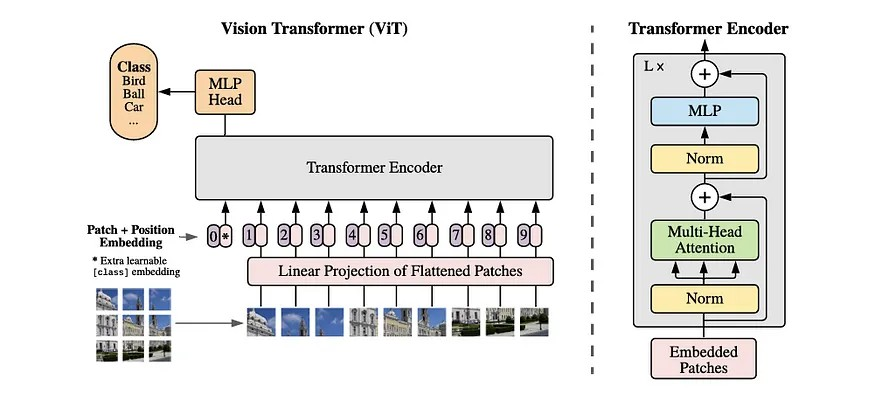
\includegraphics[width=\linewidth]{Figures/ViT.jpg}
  \caption{%
    Overview of the Vision Transformer (ViT) architecture.
    The input image is divided into fixed-size patches, which
    are flattened and projected into a sequence of patch
    embeddings.
    Positional embeddings are added to preserve spatial
    information, and a learnable classification token is
    prepended to the sequence.
    The resulting sequence is processed by a Transformer encoder
    composed of multi-head self-attention and feed-forward
    layers~\cite{dosovitskiy2020vit}.%
  }\label{fig:vit_overview}
\end{figure}


Vision Transformers (ViT) apply the Transformer model,
originally developed for natural language processing, to
computer vision tasks.
Instead of processing images through convolutional filters as in
Convolutional Neural Networks (CNNs), a ViT represents an image
as a sequence of smaller image patches.
The input image is divided into fixed-size patches
(e.g.,~$16 \times 16$ pixels), and each patch is flattened and
projected into a higher-dimensional embedding space.
Positional embeddings are then added to these patch
representations to preserve spatial information, and the
resulting sequence is processed by a Transformer encoder
composed of multi-head self-attention layers and feed-forward
networks, as described in the preceding subsections.

The output of a Vision Transformer is a set of feature
embeddings representing different spatial regions of the image,
each containing high-level semantic information.
However, because the image is divided into relatively large
patches, the resulting feature representation has a
significantly lower spatial resolution than the original input
image.
For a standard ViT with a patch size of $p = 16$, an input
image of size $H \times W$ produces a feature grid of only
$(H/p) \times (W/p)$ embeddings.
While this reduction in resolution improves computational
efficiency and encourages the model to focus on semantically
meaningful patterns, it poses a direct challenge for
dense prediction tasks such as segmentation and depth
estimation, which require high-resolution spatial outputs.
This resolution gap motivates the need for feature upsampling
techniques, discussed in the following section.

\subsection{Vision Foundation Models (VFMs)}

Vision Foundation Models are large-scale neural networks trained
on massive and diverse datasets to produce general-purpose
visual representations.
Unlike traditional task-specific models, foundation models learn
feature representations that transfer to a wide range of
downstream tasks without requiring full retraining.
They typically leverage the Vision Transformer architecture and
produce rich semantic features that capture high-level
information about image content.

Two prominent examples are DINO~\cite{caron2021dino} and CLIP~\cite{radford2021clip}\@.
DINO is a self-supervised learning method that trains Vision
Transformers without requiring labeled data.
It learns meaningful representations by encouraging consistency
between different augmented views of the same image through a
teacher--student training framework, producing features that are
particularly useful for segmentation and object discovery.
CLIP, in contrast, learns visual representations by jointly
training on large-scale image--text pairs using contrastive
learning.
By aligning visual and textual embeddings in a shared
representation space, CLIP can perform zero-shot image
classification and a wide variety of vision-language tasks.
A more recent variant, SigLIP~\cite{zhai2023siglip}, improves on CLIP by replacing
the contrastive loss with a sigmoid-based pairwise loss,
yielding stronger performance particularly at smaller batch
sizes.

Because these models are trained on massive datasets and produce
semantically rich features, they have become the dominant choice
of feature extractor in modern computer vision pipelines.
However, due to their ViT backbone, they all share the same
resolution limitation: their output feature maps are produced at
a fraction of the input resolution, making feature upsampling
an essential post-processing step for any dense prediction task.

%% ============================================================
%%  GROUP 2: Feature Upsampling
%% ============================================================
\section{Feature Upsampling}

\subsection{Interpolation-Based Methods}

Feature upsampling refers to the process of increasing the
spatial resolution of feature maps produced by deep neural
networks.
The simplest approaches rely on classical interpolation
methods, which estimate new values at higher-resolution
coordinates from the surrounding low-resolution features.

\paragraph{Nearest Neighbour Interpolation}
Each upsampled feature is copied from the nearest
low-resolution feature:
\begin{equation}
  F^{HR}(x, y)
  = F^{LR}\!\left(
      \text{round}\!\left(\tfrac{x}{s}\right),\;
      \text{round}\!\left(\tfrac{y}{s}\right)
    \right)
\end{equation}
where $s$ is the upsampling scale factor and $(x, y)$ are
coordinates in the high-resolution map.

\paragraph{Bilinear Interpolation}
Each upsampled feature is a weighted sum of the four nearest
neighbours:
\begin{equation}
  F^{HR}(x, y)
  = \sum_{i=0}^{1} \sum_{j=0}^{1}
    w_{ij}\, F^{LR}(x_i, y_j),
  \qquad
  w_{ij} = (1 - |x - x_i|)(1 - |y - y_j|)
\end{equation}

\paragraph{Bicubic Interpolation}
Bicubic interpolation uses sixteen neighbours and a cubic
kernel:
\begin{equation}
  F^{HR}(x, y)
  = \sum_{i=-1}^{2} \sum_{j=-1}^{2}
    R(i, x)\, R(j, y)\, F^{LR}(x_i, y_j)
\end{equation}
where the cubic kernel is:
\begin{equation}
  R(t) =
  \begin{cases}
    (a+2)|t|^3 - (a+3)|t|^2 + 1, & |t| \le 1 \\
    a|t|^3 - 5a|t|^2 + 8a|t| - 4a, & 1 < |t| < 2 \\
    0, & |t| \ge 2
  \end{cases}
\end{equation}
with $a = -0.5$ for the Catmull-Rom spline.

Although these methods are computationally efficient, they do
not learn how to recover spatial information lost during
downsampling, and they produce blurry or blocky results when
applied to semantic feature maps.
Learnable approaches such as transposed convolution and
sub-pixel convolution (pixel shuffle) address this by training
filters to reconstruct spatial detail from compact feature
representations.
However, all of these approaches remain task-specific and
backbone-specific, requiring retraining or retuning for each new
architecture.
This limitation motivated the development of universal,
coordinate-based upsampling methods, described next.

\subsection{Implicit Neural Representations and LIIF}

Traditional feature representations store information as
discrete grids of fixed resolution.
Implicit Neural Representations (INR) offer an alternative by
representing a signal as a continuous function parameterised by
a neural network.
Given any continuous coordinate as input, the network outputs
the corresponding value at that location, allowing the
representation to be queried at arbitrary resolutions.

Chen et al.\ (2021) applied this principle to image
super-resolution in the Local Implicit Image Function (LIIF).
An encoder produces a low-resolution feature grid from the
input image.
A decoder — implemented as a Multi-Layer Perceptron (MLP) —
then takes a target coordinate and the features of its
surrounding grid cells as input, and outputs the predicted value
at that continuous coordinate.
Because the MLP is a continuous function, the model can
generate outputs at any target resolution during inference,
including resolutions not seen during training.
This coordinate-based formulation became the conceptual
foundation for subsequent universal upsampling models,
including AnyUp.

\subsection{The AnyUp Model}

AnyUp is a state-of-the-art universal feature upsampling model
proposed by Wimmer et al.\ (2025).
Its primary contribution is the ability to upsample feature maps
from any Vision Foundation Model backbone to any target
resolution, without task-specific training or manual tuning for
each backbone.
This backbone-agnostic design is achieved through two key
architectural decisions.

First, a Feature-Agnostic Layer normalises the input feature
maps to remove statistical biases introduced by different
backbone architectures, ensuring that the decoder sees a
consistent input distribution regardless of the feature
extractor used.
Second, a Window Attention module performs the upsampling itself
by treating it as a coordinate-based retrieval problem: for each
target coordinate on the high-resolution grid, a query is formed
from the coordinate embedding and matched against local
low-resolution features using scaled dot-product attention.

AnyUp is trained using a self-supervised strategy that requires
no manual annotations.
Two views of the same image are encoded at different
resolutions; the high-resolution view serves as the
pseudo-ground-truth, and the model is trained to upsample the
low-resolution features to match it using a cosine similarity
loss:
\begin{equation}
  \mathcal{L} = 1 - \cos(\hat{f},\, f)
  \label{eq:anyup_loss}
\end{equation}
where $\hat{f}$ is the predicted high-resolution feature and $f$
is the pseudo-ground-truth.
This loss is backbone-agnostic by design, as cosine similarity
operates on normalised vectors regardless of their origin.

While AnyUp achieves strong results for static images, it
processes video sequences on a frame-by-frame basis, producing
temporally inconsistent outputs due to its complete lack of
inter-frame communication.
This limitation directly motivates the AnyUp3D framework
proposed in this thesis.

\subsection{Window-Based Attention for Upsampling}

Rather than applying attention globally across all spatial
positions — which is computationally prohibitive for
high-resolution feature maps — window-based attention restricts
the attention computation to a local neighbourhood around each
target location.
For a given query position on the high-resolution grid, only
the features within a local window of low-resolution patches
serve as keys and values.
This design dramatically reduces the computational cost of
attention-based upsampling while still providing sufficient
local context to recover fine spatial details.
Window-based attention is the core mechanism of the AnyUp model
and is retained unchanged in the AnyUp3D framework proposed
in this thesis.

%% ============================================================
%%  GROUP 3: Video Understanding and Temporal Modeling
%% ============================================================
\section{Video Understanding and Temporal Modeling}

\subsection{Temporal Consistency}

Temporal consistency refers to the property that visual
representations or predictions remain stable and coherent across
consecutive frames in a video sequence.
When a model processes each frame independently, small
variations in the input features can cause the output to vary
abruptly between adjacent frames, even when the underlying
visual content changes only slightly.
This leads to temporal artifacts such as flickering, jittering
object boundaries, and unstable semantic assignments — all of
which degrade the quality of downstream video understanding
tasks.

Temporal consistency is enforced by encouraging the model to
produce similar representations for temporally adjacent inputs.
This can be achieved through several approaches, including
temporal loss functions that penalise frame-to-frame variation,
motion cues derived from optical flow, and architectures that
explicitly model inter-frame dependencies.
In this work, temporal consistency is addressed architecturally
through the integration of 3D convolutions in the encoder and
3D cross-attention with temporal masking directly into the
upsampling pipeline, as described in Chapter~3.

\subsection{3D Convolution}

3D Convolution is a direct extension of the standard 2D
convolution operation into the temporal dimension.
A 3D convolutional kernel of size $(k \times k \times t)$ slides
simultaneously across the spatial height and width dimensions
and the temporal dimension of a video volume
$(H \times W \times T)$, extracting features that capture both
spatial appearance and temporal motion in a single unified
operation.

This joint spatial-temporal processing is more expressive than
factorised approaches that apply 2D spatial convolutions and 1D
temporal convolutions sequentially, as it can capture
correlations between motion and appearance that would otherwise
be lost.
In the proposed AnyUp3D framework, a 3D convolutional layer
with a kernel of size $3 \times 3 \times 3$ is applied to the
stacked feature volume at the early stage of the decoder, before
spatial upsampling, to extract local spatio-temporal motion
patterns from the input frame window.

\subsection{Temporal Attention}

Temporal Attention is an application of the self-attention
mechanism along the temporal axis of a video sequence.
Rather than computing attention across all spatial positions
within a single frame, temporal attention computes attention
across the same spatial position across multiple frames.
For a given pixel location $(x, y)$ in the current query frame
$t$, a query vector $Q$ is formed from the feature at that
location, while the key matrix $K$ and value matrix $V$ are
constructed from the features at the same location across all
$T$ frames in the temporal window.
The attention score for each frame is computed as the scaled
dot product between the query and the corresponding key,
followed by softmax normalisation:
\begin{equation}
  f_{\text{out}}(x,y,t)
  = \text{softmax}\!\left(
      \frac{Q_{x,y,t}\, K_{x,y,1:T}^{\top}}{\sqrt{d}}
    \right) V_{x,y,1:T}
  \label{eq:temporal_attention}
\end{equation}
The resulting output is a weighted combination of features from
all frames in the window, where frames whose content most
closely resembles the query frame receive the highest attention
weights.
This allows the model to selectively borrow stable evidence from
neighbouring frames to correct inconsistencies in the current
frame, directly suppressing flickering artifacts at the feature
level.

\subsection{Video Object Segmentation (VOS)}

Video Object Segmentation is a computer vision task that
requires identifying and delineating specific objects within
each frame of a video sequence while maintaining consistent
object identity across the full duration of the clip.
The task is typically formulated in a semi-supervised setting,
where the ground-truth segmentation mask of the target object is
provided for the first frame only, and the model must propagate
this mask through all subsequent frames.

VOS is a particularly demanding benchmark for evaluating
temporal consistency because accurate segmentation requires
stable and coherent feature representations across frames.
Any flickering or instability in the underlying feature maps
directly manifests as inconsistent or jittering segmentation
boundaries in the output masks.
For this reason, VOS is used in this work as the primary
downstream evaluation task for the AnyUp3D framework.
Performance is measured using the J\&F metric, which combines
region similarity ($\mathcal{J}$, the Jaccard index) and
contour accuracy ($\mathcal{F}$) into a single score, providing
a comprehensive measure of both spatial accuracy and boundary
sharpness.
The evaluation is conducted on the DAVIS-2017 benchmark, which
provides densely annotated video sequences covering a wide range
of challenging scenarios including fast motion, occlusion, and
appearance change.
\section*{PART II -- LITERATURE REVIEW}
\addcontentsline{toc}{section}{PART II -- LITERATURE REVIEW}

% ── Introduction ─────────────────────────────────────────────
\section{Review of Previous Studies}

The evolution of feature upsampling has transitioned from
rigid, data-independent heuristics to sophisticated,
coordinate-based neural representations.
Over the past decade, this progression has been driven by three
primary research shifts: first, the move from simple spatial
interpolation to content-aware dynamic kernels; second, the
transition from task-specific architectures to universal,
backbone-agnostic frameworks; and third, the ongoing effort to
adapt static image-based models to the temporal demands of
video sequences.

To provide a clear roadmap of this technical trajectory, the
following literature is categorised into three distinct
thematic groups:
\begin{enumerate}
  \item \textbf{Coordinate-Based and Universal Architectures:}
        Focuses on the recent shift toward treating feature maps
        as continuous functions rather than discrete grids,
        enabling arbitrary-scale upsampling across diverse model
        backbones. This group also covers the key Vision
        Foundation Models that serve as the feature extractors
        in these pipelines.

  \item \textbf{Feature Refinement and Structural Denoising:}
        Examines methodologies designed to sharpen semantic
        boundaries and remove artifacts inherent in
        Transformer-based representations.

  \item \textbf{Spatio-Temporal Stability:}
        Explores the specialised techniques developed to
        maintain visual and semantic coherence across dynamic
        video frames, including 3D convolutions, memory-based
        attention, and temporal consistency enforcement.
\end{enumerate}

% ── Group 1 ──────────────────────────────────────────────────
\subsection{Coordinate-Based and Universal Upsampling}

Chen et al.\ (2020) developed the Local Implicit Image
Function (LIIF)~\cite{liif} to overcome the fixed-scale
limitations of discrete image representations in
super-resolution tasks.
By representing images as continuous functions through a
Multi-Layer Perceptron that takes latent codes and target
coordinates as inputs, the research enabled
\textit{infinite resolution scaling}.
The study demonstrated that a single model could generalise to
arbitrary scales not encountered during training, significantly
outperforming traditional interpolation and discrete
upsamplers.
LIIF established the coordinate-based paradigm that underlies
all subsequent universal upsampling models, including those
reviewed below.

Fu et al.\ (2024) introduced FeatUp~\cite{featup}, a
task-and-model-agnostic framework that restores lost spatial
resolution in deep features produced by any Vision Foundation
Model backbone.
The methodology uses a joint bilateral upsampler that fuses
low-resolution semantic features with high-resolution guidance
from the original image through a multi-view consistency loss,
drawing analogies to Neural Radiance Fields (NeRFs).
Two variants are proposed: a fast feedforward upsampler for
general use and an implicit per-image model for arbitrary
resolution.
Crucially, the upsampled features retain their original
semantics and can be directly swapped into existing pipelines
without retraining.
FeatUp demonstrated significant improvements over bilinear
interpolation and task-specific upsamplers across class
activation mapping, segmentation, and depth prediction tasks.
However, like all image-based methods, it processes each
frame independently and produces temporally inconsistent
outputs when applied to video.

Huang et al.\ (2025) introduced LoftUp~\cite{loftup}, a
coordinate-based upsampler designed to extract high-resolution
features from Vision Foundation Models without manual labels.
The methodology utilises a cross-attention transformer to fuse
low-resolution semantic tokens with high-resolution geometric
cues from the original image.
By employing a self-supervised pseudo-ground-truth training
signal derived from class-agnostic masks, the model
successfully recovered fine-grained spatial details --- such as
thin object boundaries --- that are typically lost in
Transformer backbones.
LoftUp advances the field by demonstrating that structural
information from the original image can guide feature
upsampling more precisely than attention alone, though it
remains an image-based method with no temporal modeling
capability.

Wimmer et al.\ (2025) proposed AnyUp~\cite{anyup}, a
state-of-the-art universal upsampler designed to function
across diverse model architectures without task-specific
tuning.
The researchers implemented a feature-agnostic window attention
layer that treats upsampling as a localised re-alignment task,
mapping features from any backbone onto a higher-resolution
grid.
While the model proved superior at preserving semantic
integrity across diverse backbones, the findings highlighted a
critical limitation: its frame-by-frame processing leads to
significant temporal instability in video applications,
producing flickering artifacts at the feature level.
This limitation is the direct motivation for the AnyUp3D
framework proposed in this thesis.

Oquab et al.\ (2024) published DINOv2~\cite{dinov2}, a family
of self-supervised Vision Transformer models trained on a
large curated dataset of 142 million images.
By combining and scaling several pretraining techniques ---
including self-distillation and masked image modelling ---
DINOv2 produces all-purpose visual features that perform
competitively with weakly-supervised models across a wide range
of vision tasks, including segmentation, depth estimation, and
image retrieval, without any fine-tuning.
DINOv2 is directly relevant to this thesis as an example of the
pretrained feature extractors that the backbone-agnostic AnyUp3D
design is compatible with, alongside CLIP and SigLIP\@.
The experiments in Chapter~4 use VideoMAE as the primary feature
extractor; DINOv2, CLIP, and SigLIP represent the broader class
of Vision Foundation Models that AnyUp3D is designed to support
without task-specific retraining.

% ── Group 2 ──────────────────────────────────────────────────
\subsection{Feature Refinement and Structural Denoising}

Wang et al.\ (2019) introduced CARAFE (Content-Aware
ReAssembly of FEatures)~\cite{carafe} to replace standard,
content-blind operators such as bilinear interpolation.
The authors designed a lightweight kernel prediction module
that generates unique upsampling kernels for every spatial
location based on local context, allowing for the
content-aware reassembly of features.
The study proved that adaptive receptive fields significantly
boost performance in object detection and instance
segmentation by following the actual shapes and textures
present in an image.
CARAFE established the importance of content-awareness in
feature upsampling, but its kernels are generated from a
single backbone and cannot be directly applied across
different backbone architectures.

Yang et al.\ (2024) explored the inherent artifacts of Vision
Transformers in their work on Denoising Vision
Transformers~\cite{denoising_vit}.
By identifying that positional embeddings often cause
``checkerboard noise'' in feature maps, they proposed a
two-stage denoising method involving feature decomposition and
a learnable denoiser.
This research established a vital preprocessing step for
cleaning feature maps before upsampling, ensuring that
semantic representations remain sharp and free of structural
interference.
The findings are directly relevant to this project, since the
3D Convolution module in AnyUp3D also receives
positional-embedding-corrupted features from the backbone and
must process them reliably.

% ── Group 3 ──────────────────────────────────────────────────
\subsection{Video and Temporal Consistency}

Cheng et al.\ (2023) presented Cutie~\cite{cutie}, a video
object segmentation network that introduces object-level memory
reading to maintain consistency across frames.
The model utilises a query-based object transformer to
interact with bottom-up pixel features, allowing for
high-level semantic tracking while retaining high-resolution
feature maps.
Their methodology cleanly separated foreground semantics from
background distractors, achieving a significant improvement in
temporal stability on the MOSE dataset compared to previous
pixel-matching baselines.
Although Cutie's memory logic is optimised specifically for
video object segmentation and cannot be easily applied as a
general-purpose upsampler, its object-level temporal memory
mechanism serves as an important conceptual reference for the
temporally-extended 3D cross-attention proposed in this work.

Liu et al.\ (2022) advocated for spatio-temporal locality in
the Video Swin Transformer~\cite{swin}, extending the Swin
architecture to the 3D domain.
By implementing 3D Patch Partitioning and 3D Shifted Window
Attention, the model captures motion characteristics and
spatial relationships simultaneously.
The key finding was that joint spatio-temporal modeling
surpasses factorised models in both efficiency and accuracy,
providing a robust backbone for understanding dynamic video
content through localised 3D kernels.
Video Swin directly validates the design choice of 3D
Convolution in AnyUp3D, demonstrating that jointly
processing spatial and temporal dimensions at the feature
level leads to stronger and more coherent representations
than applying spatial and temporal operations sequentially.

Zhou et al.\ (2024) developed Upscale-A-Video~\cite{upscale_video}
to resolve the flickering artifacts common in AI-generated
video upscaling.
The project integrated 3D Convolutional layers and Temporal
Attention modules into a latent diffusion architecture to
enforce consistency across the time axis.
Their research proved that explicit temporal modeling is
essential for maintaining the coherence of moving textures,
providing a direct blueprint for the temporal extensions
proposed in this thesis.
While Upscale-A-Video is task-specific and computationally
expensive owing to its diffusion backbone, it validates the
combination of 3D convolutions and temporally-extended
cross-attention as the right architectural choices for video
feature stabilisation.

Ravi et al.\ (2024) presented Segment Anything Model 2
(SAM 2)~\cite{sam2}, a foundation model for promptable visual
segmentation in both images and videos.
SAM 2 extends the original Segment Anything Model to the
video domain by introducing a streaming memory attention
module --- a lightweight bank of object-level memories drawn
from previous frames --- that allows the model to track and
segment objects consistently across a full video sequence
in real time.
SAM 2 achieves state-of-the-art results on the DAVIS-2017
benchmark, the same evaluation dataset used in this thesis,
establishing it as the strongest contemporary baseline for
temporally consistent video segmentation.
Crucially, SAM 2's memory mechanism addresses temporal
consistency at the \emph{segmentation mask level}, while
AnyUp3D addresses the same problem at the more
fundamental \emph{feature representation level}, making the
two approaches complementary rather than competing.


% ── Comparative Analysis ─────────────────────────────────────
\section{Comparative Analysis of Previous Work}

The landscape of feature upsampling has evolved through
several technical paradigms: from fixed geometric
interpolation to content-aware dynamic kernels, and finally
toward universal, coordinate-based representations.
The primary challenge currently facing the field is what can
be termed the \textit{Universality-Stability Gap}: models
either provide high backbone flexibility without temporal
coherence, or offer temporal stability at the cost of being
architecture-locked.

The following table evaluates the key studies reviewed above
based on their technical relevance to the development of a
temporally consistent, universal upsampler.

\begin{table}[h!]
\centering
\caption{Technical Comparison of Feature Upsampling and Video
         Consistency Architectures}\label{tab:comparison}
\resizebox{\textwidth}{!}{%
\begin{tabular}{lllll}
\toprule
\textbf{Model}
  & \textbf{Domain}
  & \textbf{Backbone Compatibility}
  & \textbf{Core Strengths}
  & \textbf{Technical Weaknesses} \\
\midrule
LIIF~\cite{liif}
  & Image
  & Backbone-Agnostic
  & Infinite resolution scaling
  & Limited to RGB\@; ignores deep semantics \\
CARAFE~\cite{carafe}
  & Image
  & Task-Specific
  & Content-aware reassembly
  & Requires manual backbone tuning \\
FeatUp~\cite{featup}
  & Image
  & \textbf{Backbone-Agnostic}
  & High-res features, any backbone
  & Frame-independent; temporal jitter \\
LoftUp~\cite{loftup}
  & Image
  & Backbone-Agnostic
  & Sharpens VFM boundaries
  & No temporal modeling \\
AnyUp~\cite{anyup}
  & Image
  & \textbf{Backbone-Agnostic}
  & State-of-the-art semantic retention
  & \textbf{Zero temporal context for video} \\
Video Swin~\cite{swin}
  & Video
  & Architecture-Locked
  & Local 3D temporal context
  & Incompatible with external FM features \\
Upscale-A-Video~\cite{upscale_video}
  & Video
  & Task-Specific
  & High visual fidelity via 3D Conv
  & High compute; restricted to diffusion \\
Cutie~\cite{cutie}
  & Video
  & Task-Specific
  & Long-range object memory
  & Optimised only for segmentation masks \\
SAM 2~\cite{sam2}
  & Video
  & Task-Specific
  & Streaming memory; SOTA on DAVIS
  & Mask-level only; no feature upsampling \\
\textbf{AnyUp3D (Ours)}
  & \textbf{Video}
  & \textbf{Backbone-Agnostic}
  & \textbf{Universal + temporal consistency}
  & \textbf{Increased spatio-temporal complexity} \\
\bottomrule
\end{tabular}%
}
\end{table}

\begin{center}
  \textbf{Synthesis of Technical Relevance}
\end{center}

This comparative study highlights a critical structural void
in current upsampling methodologies.
Early learned approaches such as \textit{CARAFE} established
the superiority of content-aware upsampling over bilinear
methods but lacked the backbone compatibility required for the
diverse ecosystem of modern Vision Foundation Models.
This was addressed by coordinate-based systems such as
\textit{LIIF}, \textit{FeatUp}, and \textit{AnyUp}, which
treat feature maps as continuous functions and operate across
any backbone architecture.
While these models excel in modularity and semantic fidelity,
their independent frame processing makes them technically
insufficient for video, producing spatially accurate but
temporally disjointed features that manifest as flickering.

In contrast, dedicated video architectures such as
\textit{Video Swin}, \textit{Cutie}, and \textit{SAM 2}
provide the necessary infrastructure for temporal stability.
\textit{Video Swin} captures local motion through 3D kernels,
\textit{Cutie} introduces object-level memory reading, and
\textit{SAM 2} brings real-time streaming memory attention
for consistent video segmentation.
However, these models are fundamentally task-specific or
architecture-locked and cannot be applied as general-purpose
feature upsamplers for arbitrary backbones such as DINOv2 or
CLIP\@.

\textit{AnyUp3D} is architected to unify these two
paradigms.
By incorporating the 3D convolutional spatial-temporal modeling
of \textit{Video Swin} and the temporal attention mechanism of
\textit{Upscale-A-Video} into the backbone-agnostic framework
of \textit{AnyUp} --- realised as 3D cross-attention with
temporal masking --- we resolve the flickering artifacts found
in existing universal baselines.
This approach provides a first-of-its-kind solution that
maintains the flexibility of a Foundation Model upsampler
while enforcing the rigorous inter-frame consistency required
for high-resolution video understanding.


% ── Research Gap ─────────────────────────────────────────────
\section{Research Gap and Project Contribution}

The literature review reveals a clear dichotomy:
\begin{itemize}
  \item \textbf{Universal Upsamplers} (FeatUp, LoftUp, AnyUp)
        provide flexibility across tasks and backbones but fail
        to handle the temporal dimension, leading to
        inconsistent and flickering results in video.
  \item \textbf{Video Consistency Models}
        (Upscale-A-Video, SAM 2, Cutie) provide stability but
        are designed for specific tasks and cannot be easily
        applied as general feature upsamplers across arbitrary
        Vision Foundation Model backbones.
\end{itemize}

\textbf{Project Contribution:}
This project addresses this gap by proposing
\textit{AnyUp3D}.
We contribute a novel architecture that integrates the
\emph{temporal stability} mechanisms of video models ---
specifically 3D convolutions in the encoder (validated by
\textit{Video Swin}) and 3D cross-attention with temporal masking
(validated by \textit{Upscale-A-Video}) --- into the
\emph{universal framework} of AnyUp.
This yields the first task-agnostic, backbone-agnostic feature
upsampler capable of producing temporally consistent results
for video sequences.




